\documentclass{article}
\usepackage[utf8]{inputenc}
\usepackage{graphicx}
\usepackage{listings}
\usepackage[dvipsnames]{xcolor}
\usepackage{amsmath}
\usepackage{hyperref}
\usepackage{subcaption}
\usepackage{array}
\usepackage{geometry}
\newcommand{\sectionlinetwo}[2]{%
\nointerlineskip \vspace{.5\baselineskip}\hspace{\fill}
  {\color{#1}
    \resizebox{0.5\linewidth}{2ex}
    {{%
    {\begin{tikzpicture}
    \node  (C) at (0,0) {};
    \node (D) at (9,0) {};
    \path (C) to [ornament=#2] (D);
    \end{tikzpicture}}}}}%
    \hspace{\fill}
    \par\nointerlineskip \vspace{.5\baselineskip}
  }
\geometry{
 a4paper,
 total={170mm,257mm},
 left=20mm,
 top=20mm,
 }
\definecolor{azure}{rgb}{0.0, 0.5, 1.0}
\definecolor{forestgreen}{rgb}{0.13, 0.55, 0.13}
\definecolor{codegreen}{rgb}{0,0.6,0}
\definecolor{codegray}{rgb}{0.5,0.5,0.5}
\definecolor{codepurple}{rgb}{0.58,0,0.82}
\definecolor{backcolour}{rgb}{0.95,0.95,0.92}

\lstdefinestyle{mystyle}{
    backgroundcolor=\color{backcolour},   
    commentstyle=\color{codegreen},
    keywordstyle=\color{magenta},
    numberstyle=\tiny\color{codegray},
    stringstyle=\color{codepurple},
    basicstyle=\ttfamily\footnotesize,
    breakatwhitespace=false,         
    breaklines=true,                 
    captionpos=b,                    
    keepspaces=true,                 
    numbers=left,                    
    numbersep=5pt,                  
    showspaces=false,                
    showstringspaces=false,
    showtabs=false,                  
    tabsize=2
}
\lstset{style=mystyle}

\title{Submission for Programming Assignment 1\\\small{\textit{CS 427: Mathematics for Data Science, Autumn 2020-21}}}
\author{Group 9: K. Sai Anuroop (170030035), Rohan Savakar (170030033)}
\date{\today}

\begin{document}
    \maketitle
    \begin{flushleft}
        The code performs Principal Component Analysis on the set of images provided to us from Olivetti faces dataset. It then randomly chooses an image, reconstructs it using $4096$ components, $x$ components and $<x$ components, where $x$ is provided as an input argument by the user. We interpret $x$ as the minimum number of components required to reconstruct the image such that the face of the person is discernible.\\
        Below is an exhaustive list of all the $30$ images provided to us along with their reconstructed counterparts as per the scheme mentioned above.\\
        \begin{table}[h!]
            \centering
            \begin{tabular}{ | c | c | c | c |}
                \hline
                Original & $4096$ & $x$ & $<x$ \\ \hline\hline
                \raisebox{.17\height}{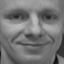
\includegraphics[width=1.7cm]{0.png}} & 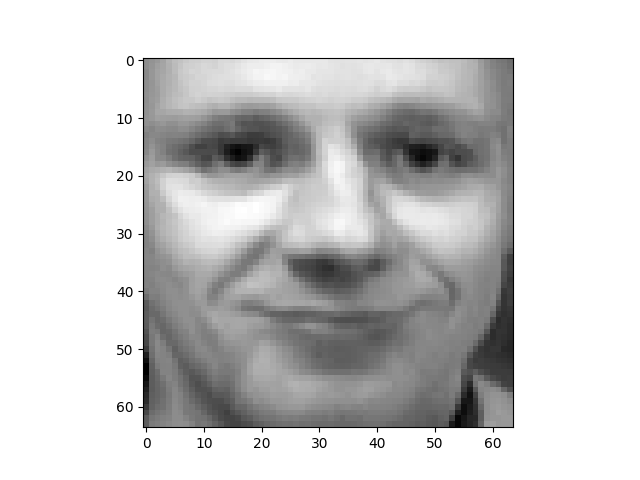
\includegraphics[width=3cm]{./output/img0/4096pc_recon_0.png} & 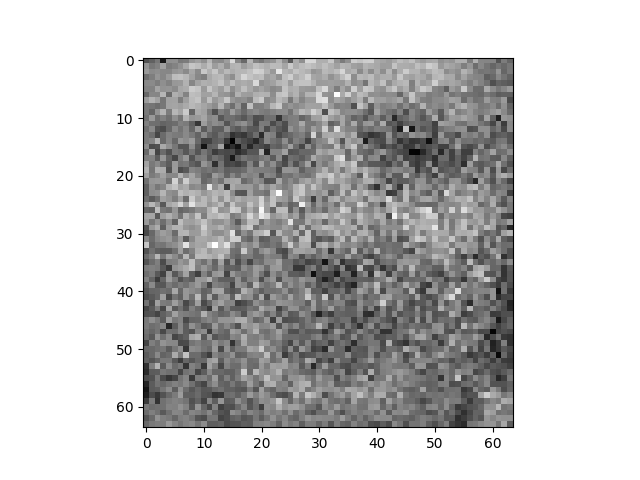
\includegraphics[width=3cm]{./output/img0/3100pc_recon_0.png} & 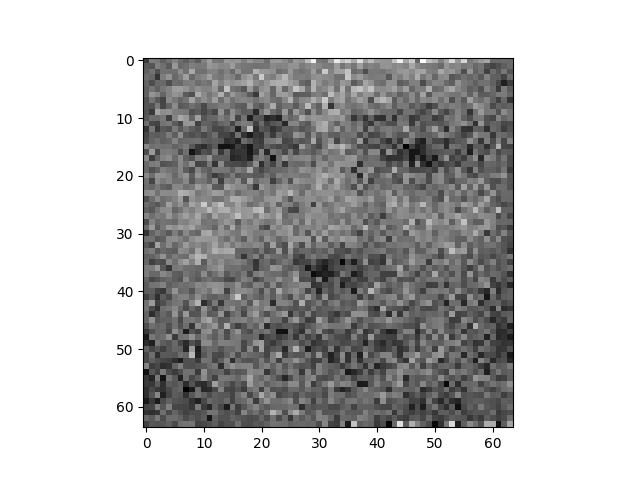
\includegraphics[width=3cm]{./output/img0/353pc_recon_0.png}\\
                0.png & - & 3100 & 353 \\ \hline
                \raisebox{.17\height}{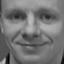
\includegraphics[width=1.7cm]{1.png}} & 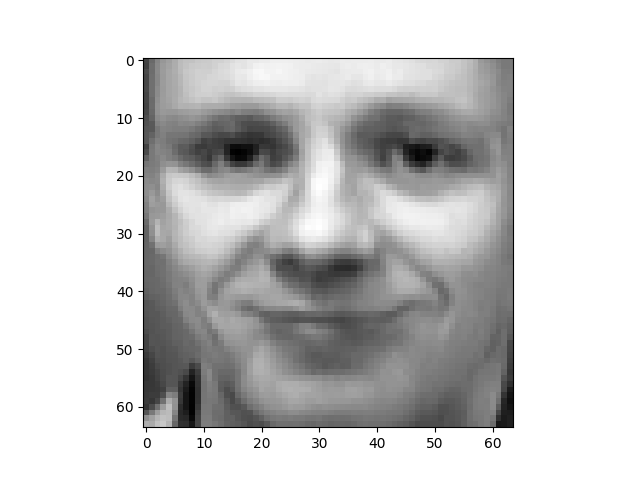
\includegraphics[width=3cm]{./output/img1/4096pc_recon_1.png} & 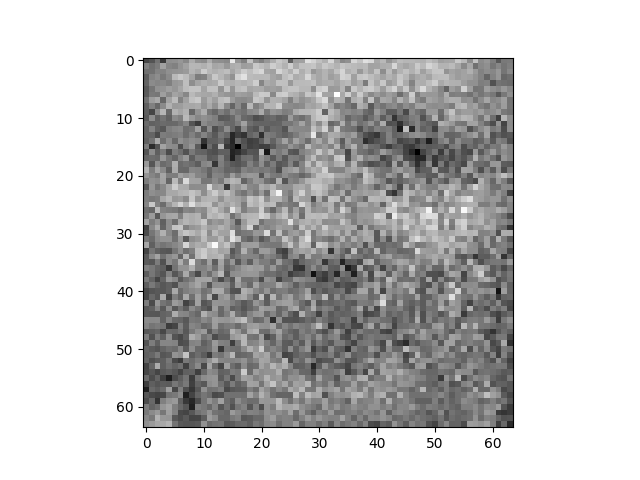
\includegraphics[width=3cm]{./output/img1/3250pc_recon_1.png} & 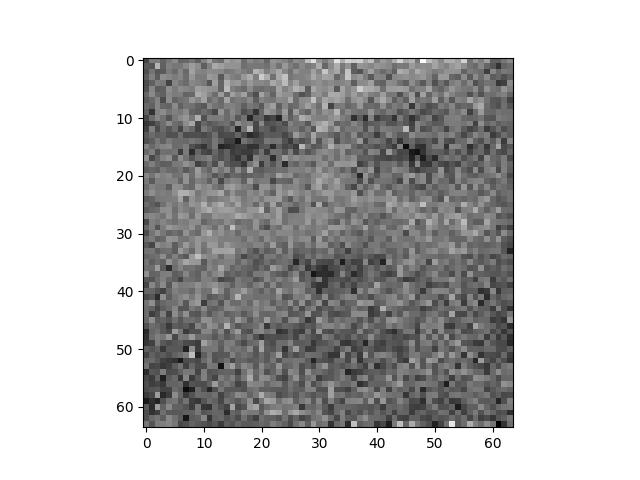
\includegraphics[width=3cm]{./output/img1/476pc_recon_1.png}\\
                1.png & - & 3250 & 476 \\ \hline
                \raisebox{.17\height}{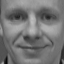
\includegraphics[width=1.7cm]{2.png}} & 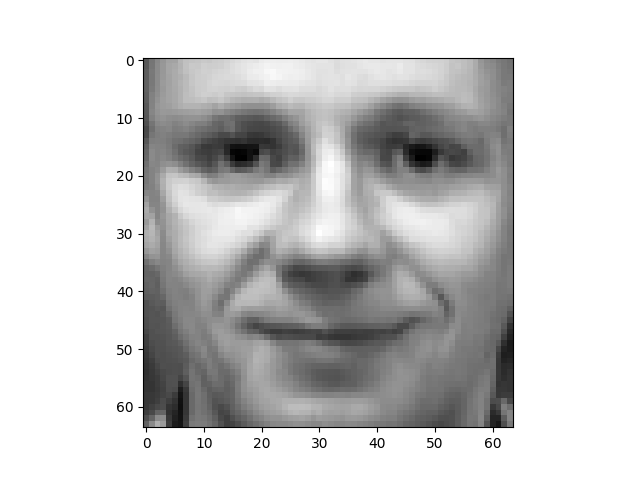
\includegraphics[width=3cm]{./output/img2/4096pc_recon_2.png} & 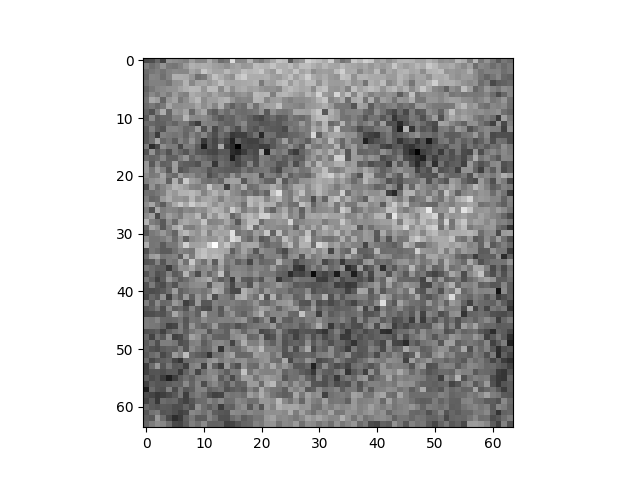
\includegraphics[width=3cm]{./output/img2/3300pc_recon_2.png} & 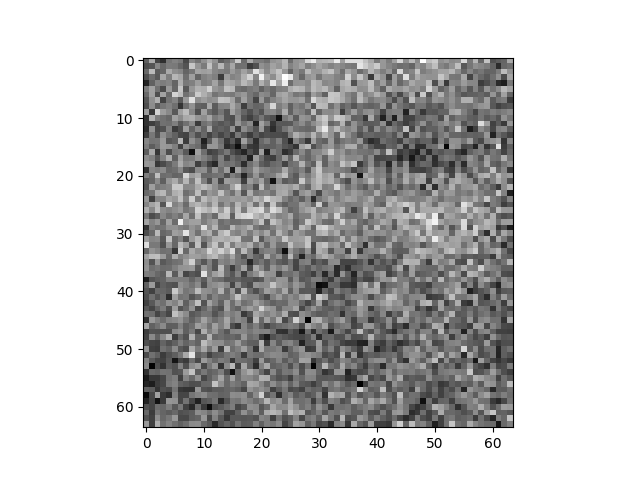
\includegraphics[width=3cm]{./output/img2/1220pc_recon_2.png}\\
                2.png & - & 3300 & 1220 \\ \hline
                \raisebox{.17\height}{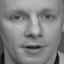
\includegraphics[width=1.7cm]{3.png}} & 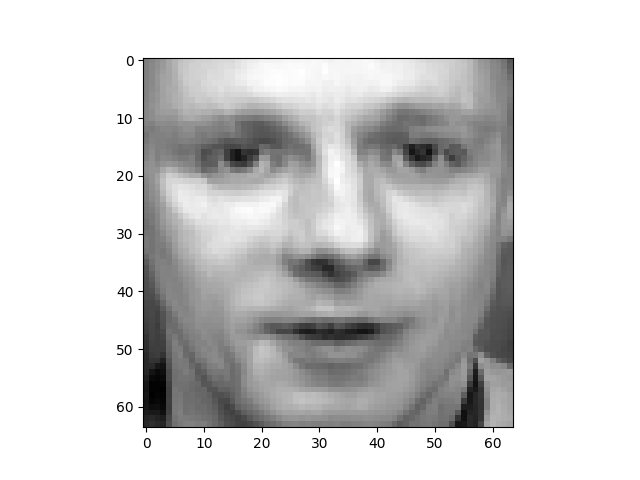
\includegraphics[width=3cm]{./output/img3/4096pc_recon_3.png} & 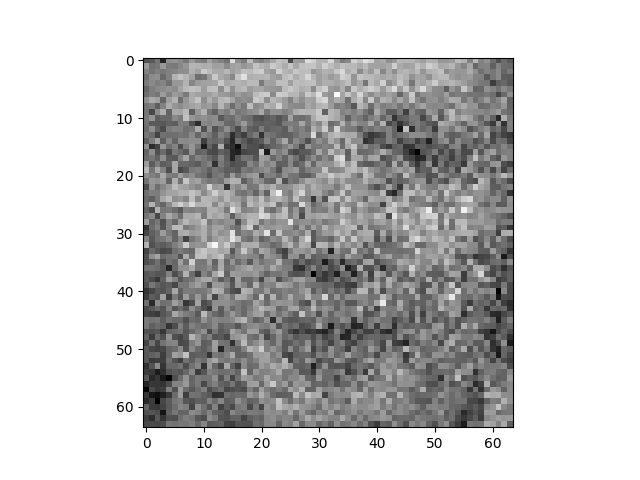
\includegraphics[width=3cm]{./output/img3/3250pc_recon_3.png} & 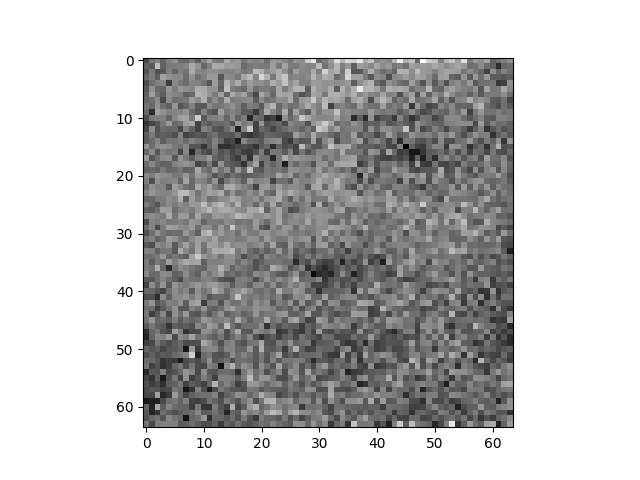
\includegraphics[width=3cm]{./output/img3/476pc_recon_3.png}\\
                3.png & - & 3250 & 476 \\ \hline
                \raisebox{.17\height}{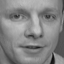
\includegraphics[width=1.7cm]{4.png}} & 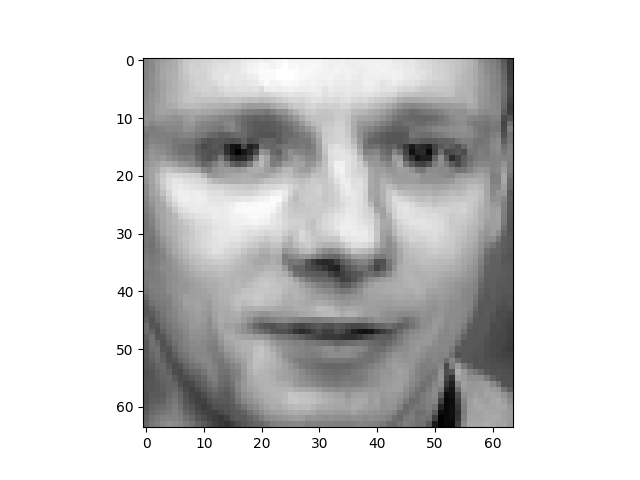
\includegraphics[width=3cm]{./output/img4/4096pc_recon_4.png} & 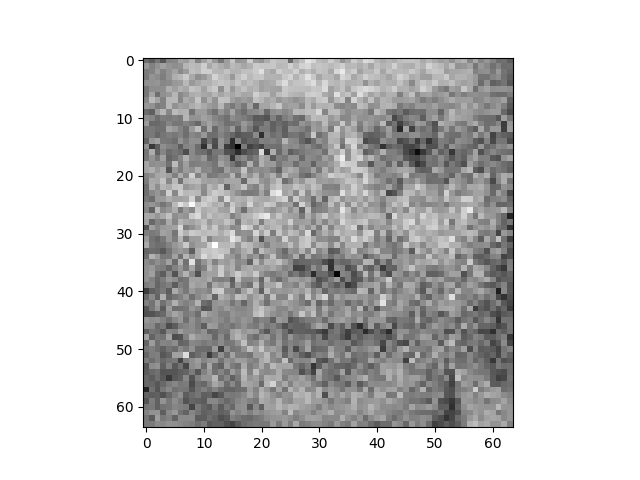
\includegraphics[width=3cm]{./output/img4/3500pc_recon_4.png} & 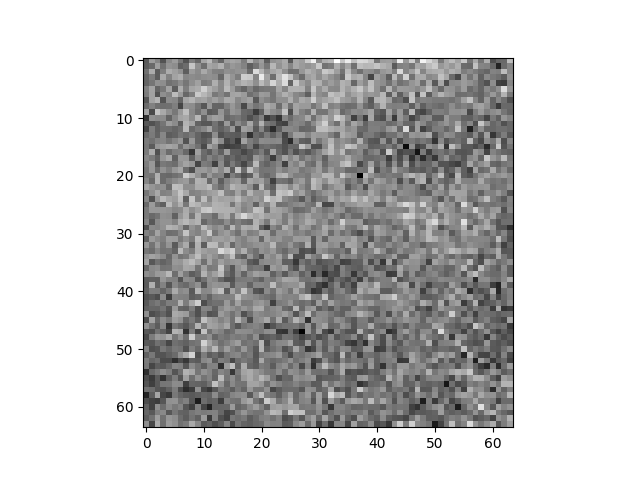
\includegraphics[width=3cm]{./output/img4/817pc_recon_4.png}\\
                4.png & - & 3500 & 817 \\ \hline
                \raisebox{.17\height}{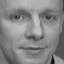
\includegraphics[width=1.7cm]{5.png}} & 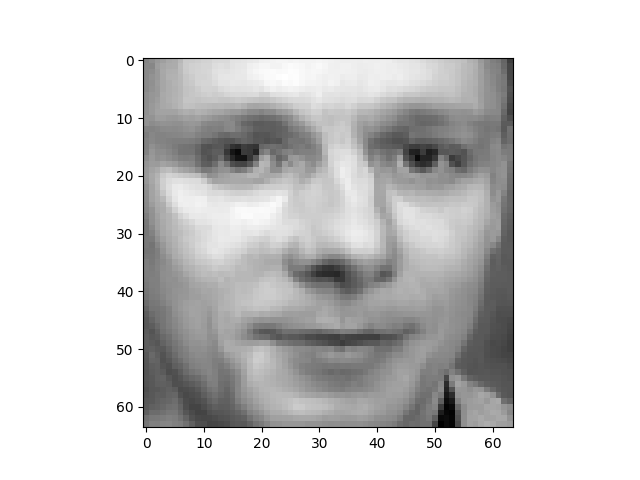
\includegraphics[width=3cm]{./output/img5/4096pc_recon_5.png} & 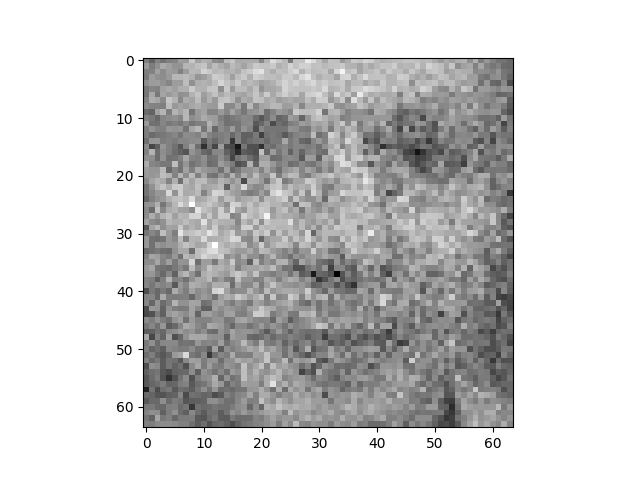
\includegraphics[width=3cm]{./output/img5/3650pc_recon_5.png} & 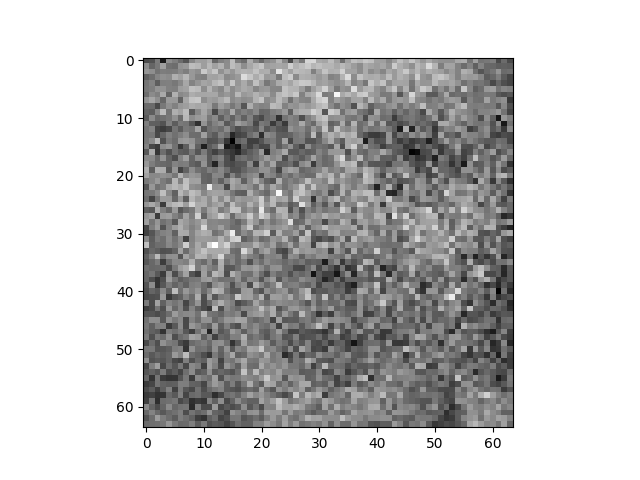
\includegraphics[width=3cm]{./output/img5/2990pc_recon_5.png}\\
                5.png & - & 3650 & 2990 \\ \hline
            \end{tabular}
        \end{table}
        \clearpage
        \begin{table}[h!]
            \centering
            \begin{tabular}{ | c | c | c | c |}
                \hline
                Original & $4096$ & $x$ & $<x$ \\ \hline\hline
                \raisebox{.17\height}{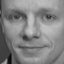
\includegraphics[width=1.7cm]{6.png}} & 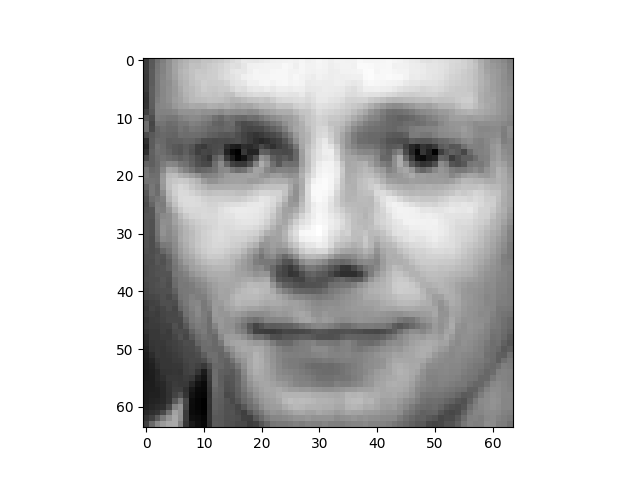
\includegraphics[width=3cm]{./output/img6/4096pc_recon_6.png} & 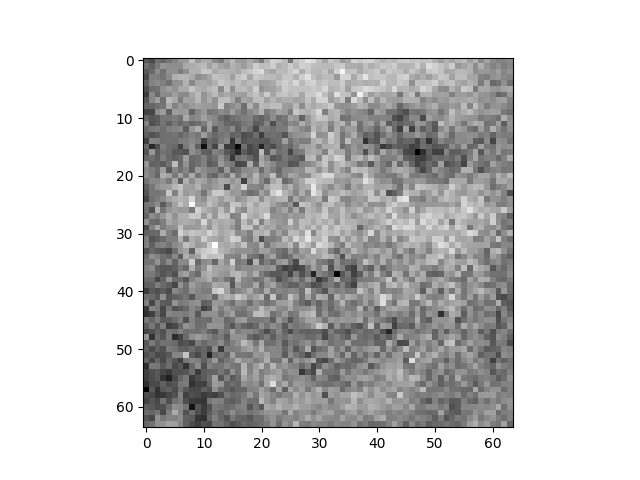
\includegraphics[width=3cm]{./output/img6/3650pc_recon_6.png} & 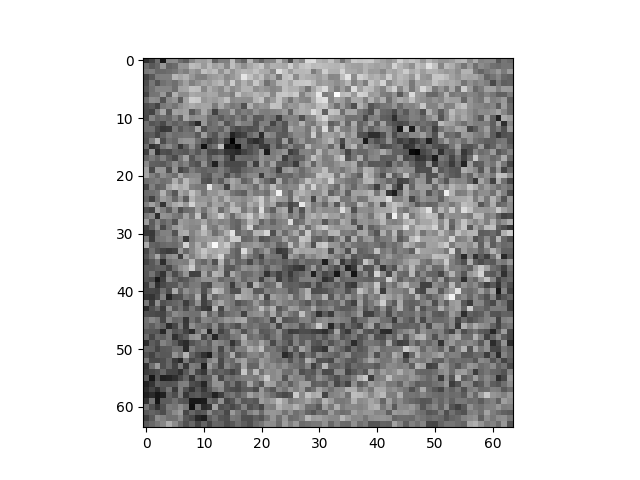
\includegraphics[width=3cm]{./output/img6/2990pc_recon_6.png}\\
                6.png & - & 3650 & 2990 \\ \hline
                \raisebox{.17\height}{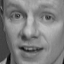
\includegraphics[width=1.7cm]{7.png}} & 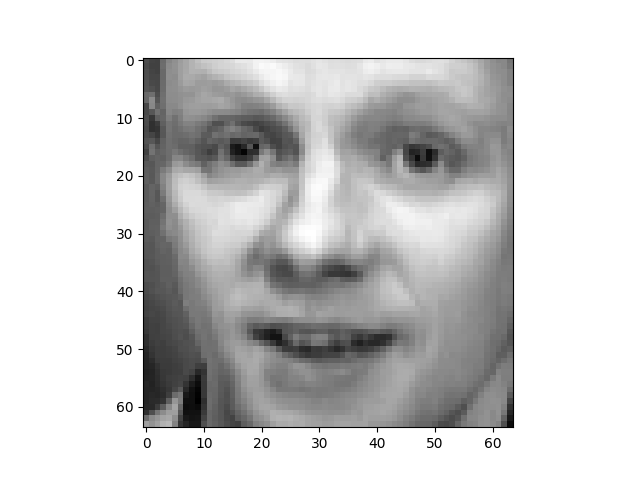
\includegraphics[width=3cm]{./output/img7/4096pc_recon_7.png} & 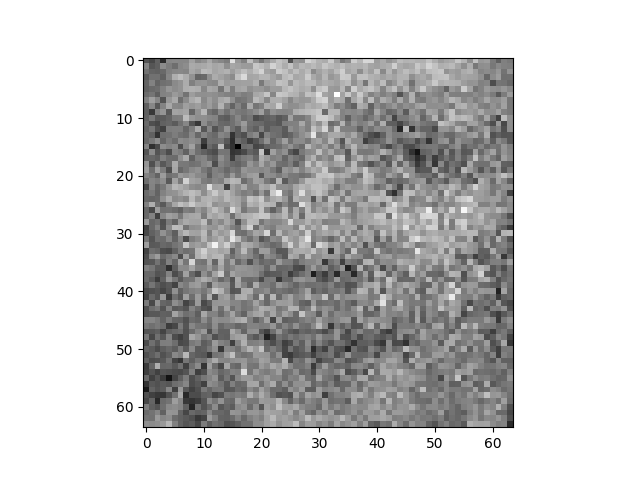
\includegraphics[width=3cm]{./output/img7/3250pc_recon_7.png} & 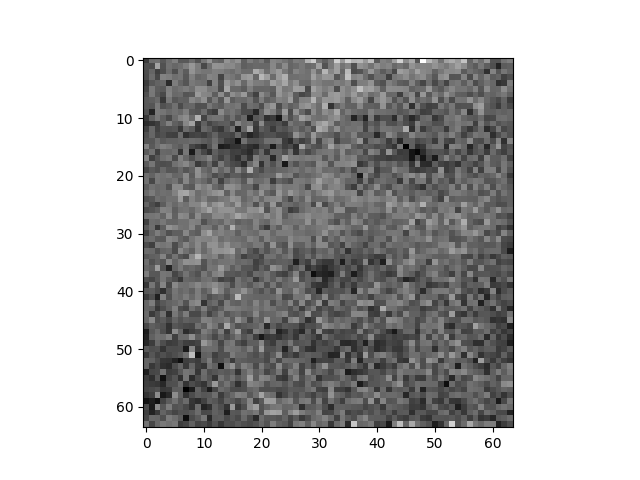
\includegraphics[width=3cm]{./output/img7/476pc_recon_7.png}\\
                7.png & - & 3250 & 476 \\ \hline
                \raisebox{.17\height}{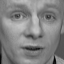
\includegraphics[width=1.7cm]{8.png}} & 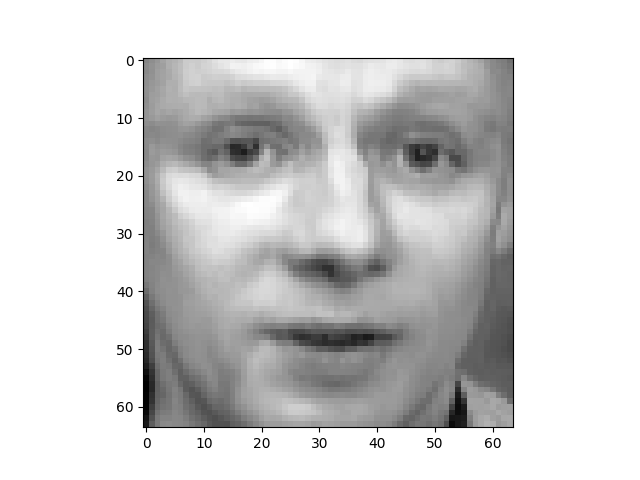
\includegraphics[width=3cm]{./output/img8/4096pc_recon_8.png} & 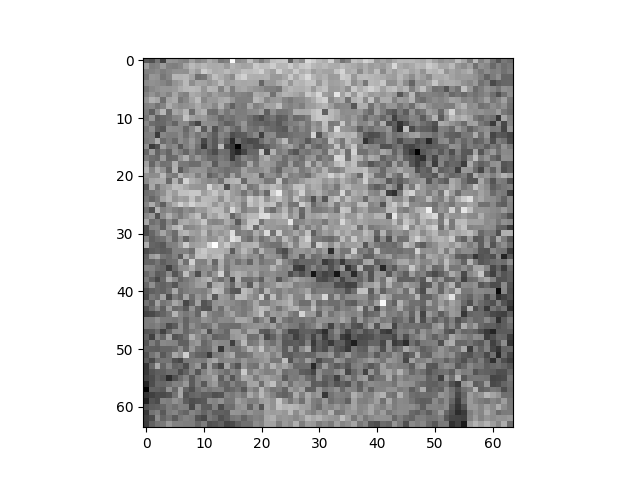
\includegraphics[width=3cm]{./output/img8/3300pc_recon_8.png} & 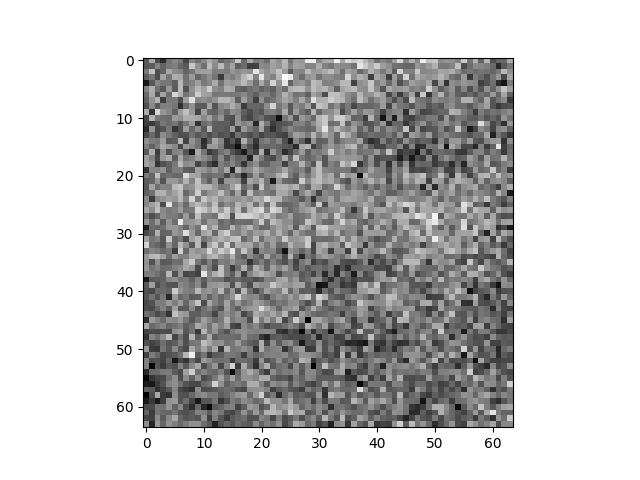
\includegraphics[width=3cm]{./output/img8/1220pc_recon_8.png}\\
                8.png & - & 3300 & 1220 \\ \hline
                \raisebox{.17\height}{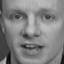
\includegraphics[width=1.7cm]{9.png}} & 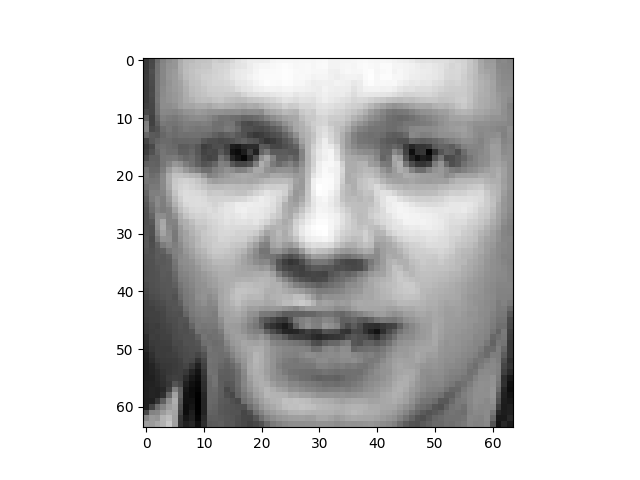
\includegraphics[width=3cm]{./output/img9/4096pc_recon_9.png} & 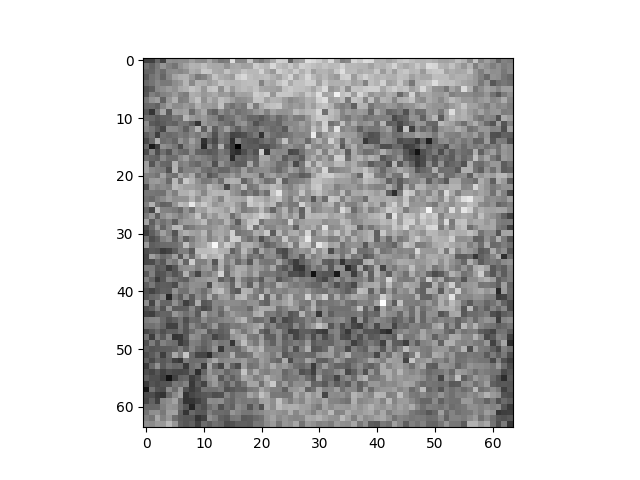
\includegraphics[width=3cm]{./output/img9/3350pc_recon_9.png} & 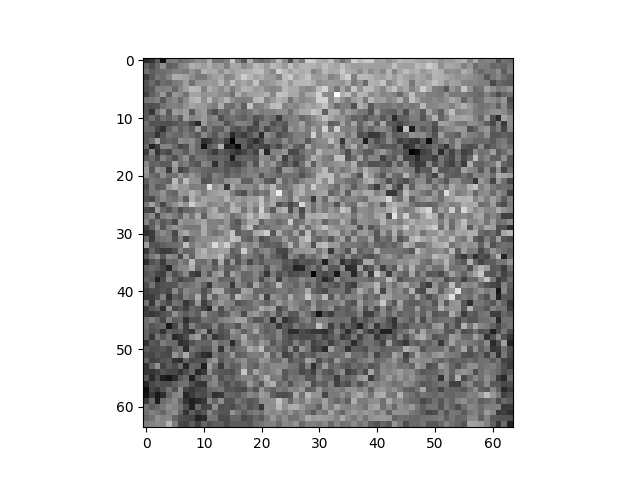
\includegraphics[width=3cm]{./output/img9/3105pc_recon_9.png}\\
                9.png & - & 3350 & 3105 \\ \hline
                \raisebox{.17\height}{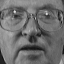
\includegraphics[width=1.7cm]{10.png}} & 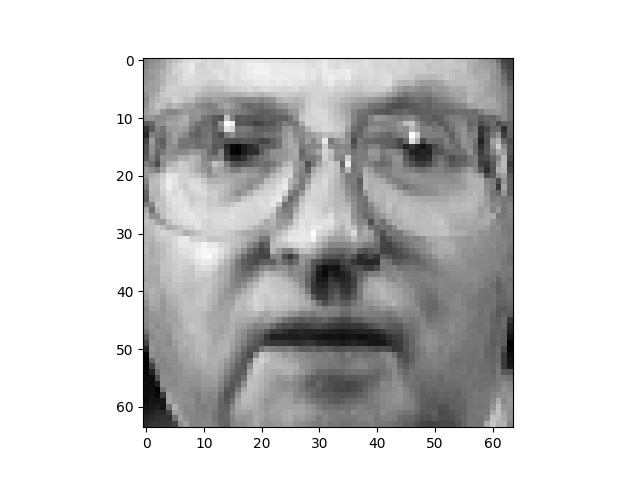
\includegraphics[width=3cm]{./output/img10/4096pc_recon_10.png} & 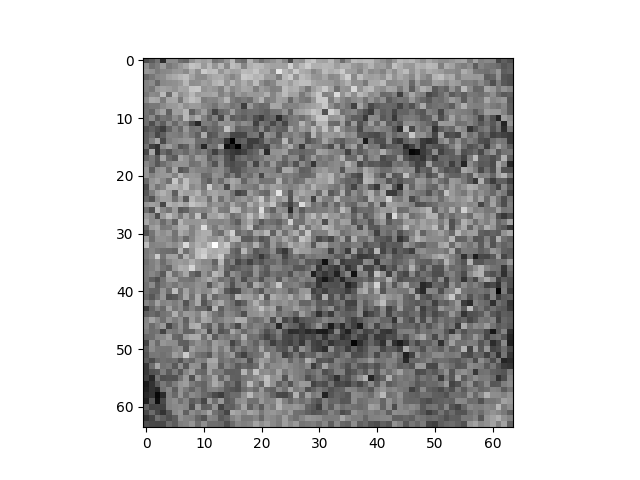
\includegraphics[width=3cm]{./output/img10/3000pc_recon_10.png} & 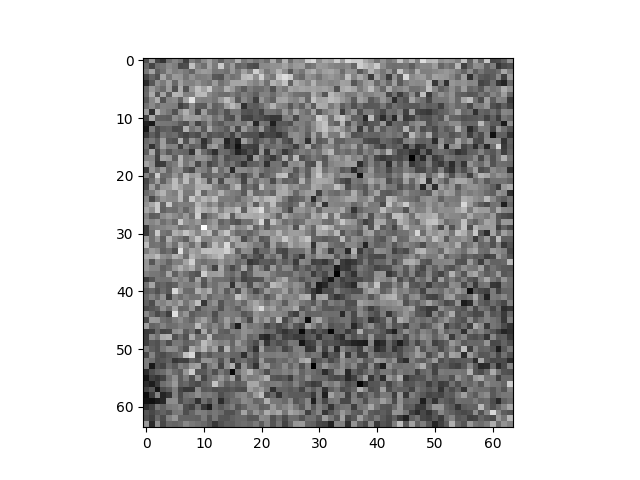
\includegraphics[width=3cm]{./output/img10/1331pc_recon_10.png}\\
                10.png & - & 3000 & 1331 \\ \hline
                \raisebox{.17\height}{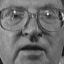
\includegraphics[width=1.7cm]{11.png}} & 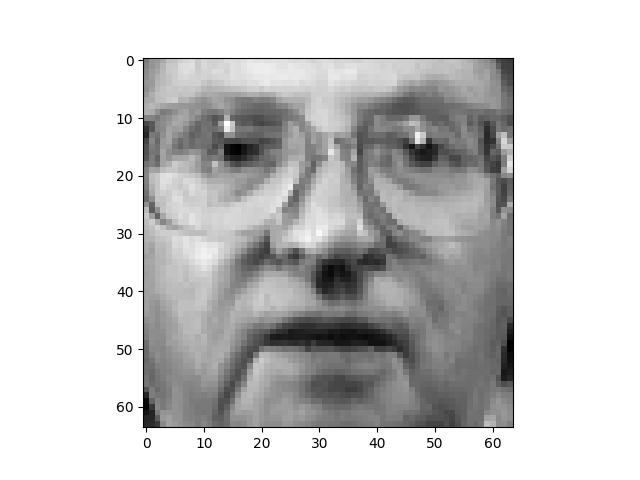
\includegraphics[width=3cm]{./output/img11/4096pc_recon_11.png} & 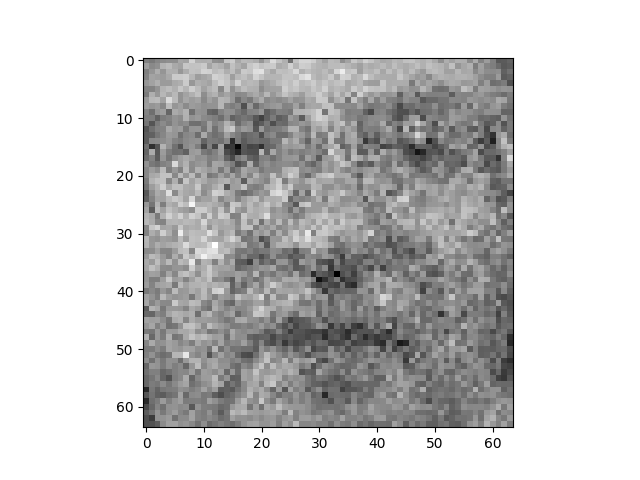
\includegraphics[width=3cm]{./output/img11/3650pc_recon_11.png} & 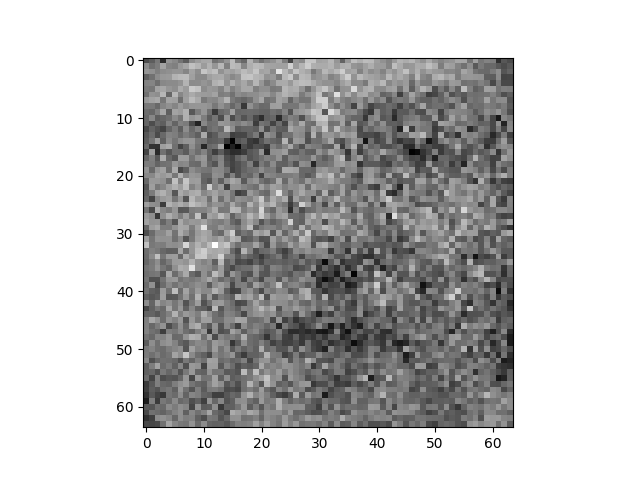
\includegraphics[width=3cm]{./output/img11/2990pc_recon_11.png}\\
                11.png & - & 3650 & 2990 \\ \hline
                \raisebox{.17\height}{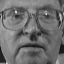
\includegraphics[width=1.7cm]{12.png}} & 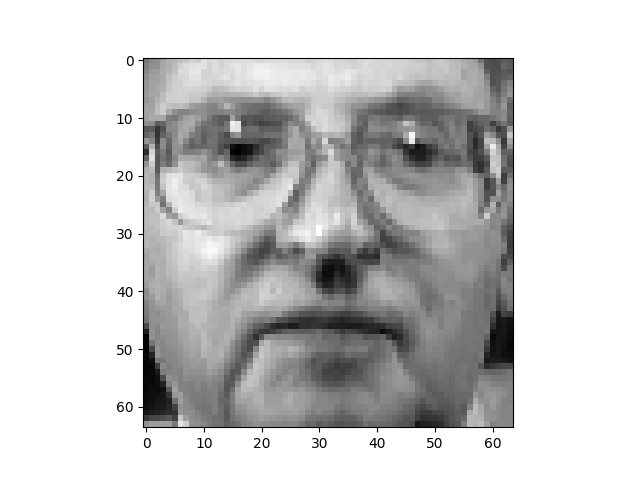
\includegraphics[width=3cm]{./output/img12/4096pc_recon_12.png} & \includegraphics[width=3cm]{./output/img12/3050pc_recon_12.png} & \includegraphics[width=3cm]{./output/img12/541pc_recon_12.png}\\
                12.png & - & 3050 & 541 \\ \hline
                \raisebox{.17\height}{\includegraphics[width=1.7cm]{13.png}} & \includegraphics[width=3cm]{./output/img13/4096pc_recon_13.png} & \includegraphics[width=3cm]{./output/img13/3200pc_recon_13.png} & \includegraphics[width=3cm]{./output/img13/2098pc_recon_13.png}\\
                13.png & - & 3200 & 2098 \\ \hline
                \raisebox{.17\height}{\includegraphics[width=1.7cm]{14.png}} & \includegraphics[width=3cm]{./output/img14/4096pc_recon_14.png} & \includegraphics[width=3cm]{./output/img14/3200pc_recon_14.png} & \includegraphics[width=3cm]{./output/img14/2098pc_recon_14.png}\\
                14.png & - & 3200 & 2098 \\ \hline
            \end{tabular}
        \end{table}
        \clearpage
        \begin{table}[h!]
            \centering
            \begin{tabular}{ | c | c | c | c |}
                \hline
                Original & $4096$ & $x$ & $<x$ \\ \hline\hline
                \raisebox{.17\height}{\includegraphics[width=1.7cm]{15.png}} & \includegraphics[width=3cm]{./output/img15/4096pc_recon_15.png} & \includegraphics[width=3cm]{./output/img15/3100pc_recon_15.png} & \includegraphics[width=3cm]{./output/img15/353pc_recon_15.png}\\
                15.png & - & 3100 & 353 \\ \hline
                \raisebox{.17\height}{\includegraphics[width=1.7cm]{16.png}} & \includegraphics[width=3cm]{./output/img16/4096pc_recon_16.png} & \includegraphics[width=3cm]{./output/img16/3000pc_recon_16.png} & \includegraphics[width=3cm]{./output/img16/1331pc_recon_16.png}\\
                16.png & - & 3000 & 1331 \\ \hline
                \raisebox{.17\height}{\includegraphics[width=1.7cm]{17.png}} & \includegraphics[width=3cm]{./output/img17/4096pc_recon_17.png} & \includegraphics[width=3cm]{./output/img17/3200pc_recon_17.png} & \includegraphics[width=3cm]{./output/img17/2098pc_recon_17.png}\\
                17.png & - & 3200 & 2098 \\ \hline
                \raisebox{.17\height}{\includegraphics[width=1.7cm]{18.png}} & \includegraphics[width=3cm]{./output/img18/4096pc_recon_18.png} & \includegraphics[width=3cm]{./output/img18/3100pc_recon_18.png} & \includegraphics[width=3cm]{./output/img18/353pc_recon_18.png}\\
                18.png & - & 3100 & 353 \\ \hline
                \raisebox{.17\height}{\includegraphics[width=1.7cm]{19.png}} & \includegraphics[width=3cm]{./output/img19/4096pc_recon_19.png} & \includegraphics[width=3cm]{./output/img19/3050pc_recon_19.png} & \includegraphics[width=3cm]{./output/img19/541pc_recon_19.png}\\
                19.png & - & 3050 & 541 \\ \hline
                \raisebox{.17\height}{\includegraphics[width=1.7cm]{20.png}} & \includegraphics[width=3cm]{./output/img20/4096pc_recon_20.png} & \includegraphics[width=3cm]{./output/img20/3000pc_recon_20.png} & \includegraphics[width=3cm]{./output/img20/1331pc_recon_20.png}\\
                20.png & - & 3000 & 1331 \\ \hline
                \raisebox{.17\height}{\includegraphics[width=1.7cm]{21.png}} & \includegraphics[width=3cm]{./output/img21/4096pc_recon_21.png} & \includegraphics[width=3cm]{./output/img21/2700pc_recon_21.png} & \includegraphics[width=3cm]{./output/img21/1587pc_recon_21.png}\\
                21.png & - & 2700 & 1587 \\ \hline
                \raisebox{.17\height}{\includegraphics[width=1.7cm]{22.png}} & \includegraphics[width=3cm]{./output/img22/4096pc_recon_22.png} & \includegraphics[width=3cm]{./output/img22/2700pc_recon_22.png} & \includegraphics[width=3cm]{./output/img22/1587pc_recon_22.png}\\
                22.png & - & 2700 & 1587 \\ \hline
            \end{tabular}
        \end{table}
        \clearpage
        \begin{table}[h!]
            \centering
            \begin{tabular}{ | c | c | c | c |}
                \hline
                Original & $4096$ & $x$ & $<x$ \\ \hline\hline
                \raisebox{.17\height}{\includegraphics[width=1.7cm]{23.png}} & \includegraphics[width=3cm]{./output/img23/4096pc_recon_23.png} & \includegraphics[width=3cm]{./output/img23/3000pc_recon_23.png} & \includegraphics[width=3cm]{./output/img23/1331pc_recon_23.png}\\
                23.png & - & 3000 & 1331 \\ \hline
                \raisebox{.17\height}{\includegraphics[width=1.7cm]{24.png}} & \includegraphics[width=3cm]{./output/img24/4096pc_recon_24.png} & \includegraphics[width=3cm]{./output/img24/2700pc_recon_24.png} & \includegraphics[width=3cm]{./output/img24/1587pc_recon_24.png}\\
                24.png & - & 2700 & 1587 \\ \hline
                \raisebox{.17\height}{\includegraphics[width=1.7cm]{25.png}} & \includegraphics[width=3cm]{./output/img25/4096pc_recon_25.png} & \includegraphics[width=3cm]{./output/img25/2750pc_recon_25.png} & \includegraphics[width=3cm]{./output/img25/523pc_recon_25.png}\\
                25.png & - & 2750 & 523 \\ \hline
                \raisebox{.17\height}{\includegraphics[width=1.7cm]{26.png}} & \includegraphics[width=3cm]{./output/img26/4096pc_recon_26.png} & \includegraphics[width=3cm]{./output/img26/2900pc_recon_26.png} & \includegraphics[width=3cm]{./output/img26/1744pc_recon_26.png}\\
                26.png & - & 2900 & 1744 \\ \hline
                \raisebox{.17\height}{\includegraphics[width=1.7cm]{27.png}} & \includegraphics[width=3cm]{./output/img27/4096pc_recon_27.png} & \includegraphics[width=3cm]{./output/img27/2900pc_recon_27.png} & \includegraphics[width=3cm]{./output/img27/1744pc_recon_27.png}\\
                27.png & - & 2900 & 1744 \\ \hline
                \raisebox{.17\height}{\includegraphics[width=1.7cm]{28.png}} & \includegraphics[width=3cm]{./output/img28/4096pc_recon_28.png} & \includegraphics[width=3cm]{./output/img28/2850pc_recon_28.png} & \includegraphics[width=3cm]{./output/img28/2450pc_recon_28.png}\\
                28.png & - & 2850 & 2450 \\ \hline
                \raisebox{.17\height}{\includegraphics[width=1.7cm]{29.png}} & \includegraphics[width=3cm]{./output/img29/4096pc_recon_29.png} & \includegraphics[width=3cm]{./output/img29/2700pc_recon_29.png} & \includegraphics[width=3cm]{./output/img29/1587pc_recon_29.png}\\
                29.png & - & 2700 & 1587 \\ \hline
            \end{tabular}
        \end{table}
        $3005$ is the average of all the values of $x$ listed in the above table, which we consider to be the value of $x$ that is required to discern the faces, according to our discretion.  
        \clearpage
        \begin{lstlisting}[language=Python, title={Python code to perform PCA on images}]
"""
This code performs PCA on the set of images provided in the format <number>.png,
reconstructs a randomly chosen image from the input set using [4096, k, <k] Principal Components,
and saves in ./output/img<number> directory.
Note that this code has to be placed in the same directory as the set of input images (or else change the path in the code accordingly)
"""
import os
import sys
import numpy as np
import pandas as pd
import random
import matplotlib.pyplot as plt
import matplotlib.image as mpimg
from sklearn.decomposition import PCA
from glob import iglob
from numpy import mean
from numpy import cov
from numpy.linalg import eigh
from pathlib import Path

# checking if sufficient input arguments are provided and if provided, are correct or not
if(len(sys.argv)<2 or int(sys.argv[1])>4096 or int(sys.argv[1])<1):
    print("Usage: python3 pca3.py <num_principal_components_to_retain>")
    print("Note: 1 <= num_principal_components_to_retain <= 4096")
    exit(1)

# dataframes to store images of a person's face
faces_0 = pd.DataFrame([])
faces_1 = pd.DataFrame([])
faces_2 = pd.DataFrame([])
all_faces = pd.DataFrame([])

# convert 64*64 images to a pandas dataframe of 4096 size each
for path in iglob("*.png"):
    img=mpimg.imread(path)
    # print(int(''.join(path.split('.')[0])))
    face = pd.Series(img.flatten(),name=path)
    all_faces = all_faces.append(face)
    if int(int(path[0:path.find('.')])/10)==0:
        # print(int(path[0:path.find('.')]))
        faces_0 = faces_0.append(face)
    elif int(int(path[0:path.find('.')])/10)==1:
        # print(int(path[0:path.find('.')]))
        faces_1 = faces_1.append(face)
    else:
        # print(int(path[0:path.find('.')]))
        faces_2 = faces_2.append(face)

# uncomment to choose a random person to perform PCA on the set of images of "that" person
"""
# choose a random person to perform PCA
face_num = random.randint(0,((len(faces_0)+len(faces_1)+len(faces_2))/10)-1)
# choose a random image of the person to compare with
which_face = random.randint(0,10)
fit_which_face = faces_0
if face_num == 0:
    fit_which_face = faces_0
    my_face = faces_0[which_face]
elif face_num == 1:
    fit_which_face = faces_1
    my_face = faces_1[which_face]
else:
    fit_which_face = faces_2
    my_face = faces_2[which_face]
"""
# sort indices of images
all_faces = all_faces.assign(indexNumber=[int(''.join(i.split('.')[0])) for i in all_faces.index])
all_faces.sort_values(['indexNumber'], ascending = [True], inplace = True)
all_faces.drop('indexNumber', 1, inplace = True)

temp = all_faces # temp: 30 x 4096
temp = temp.values
mean_matrix = mean(temp.T, axis=1)
centred_matrix = temp - mean_matrix
cov_matrix = cov(centred_matrix.T) # finding covariance matrix
values, vectors = eigh(cov_matrix) # finding eigenvectors (Principal Components) of covariance matrix
vectors = np.real(vectors) # vectors: 4096 x 4096

# sort eigenvectors (Principal Components) based on their eigenvalues in descending order
idx = values.argsort()[::-1]
values = values[idx]
vectors = vectors[:,idx]

retention_vector = [4096, int(sys.argv[1]), random.randint(0,int(sys.argv[1]))] # array storing number of eigevectors (Principal Components) to be used while reconstructing image
# choose an image to reconstruct and create an output directory for the same
reconstruct_img_num = random.randint(0,29)
# reconstruct_img_num = 18
filename = "./output/img"+str(reconstruct_img_num)
Path(filename).mkdir(parents=True, exist_ok=True)

for k in retention_vector: # reconstruct the chosen image using [4096, k, <k] eigevectors (Principal Components)
    # retain only k eigevectors (Principal Components)
    retained_values = values[:k] # choose this number k
    retained_vectors = vectors[:k] # retained_vectors: k x 4096

    # Summary of matrix dimensions
    # temp: 30 x 4096
    # retained_vectors: k x 4096
    # projected_matrix: 30 x k
    # recon_matrix: 30 x 4096

    # reconstruct images
    projected_matrix = temp.dot(retained_vectors.T) # projected_matrix: 30 x k
    recon_matrix = projected_matrix.dot(retained_vectors)+mean_matrix # recon_matrix: 30 x 4096
    plt.imshow(recon_matrix[reconstruct_img_num].reshape(64,64),cmap="gray")
    plt.savefig(filename+"/"+str(k)+"pc_recon_"+str(reconstruct_img_num)+".png")
        \end{lstlisting}
        \clearpage
        \begin{figure}[htp]
                \centering
                \includegraphics[width=9cm]{./qr/qr-code.png}\\
                Scan this QR code to access the GitHub repository of my homweork solutions at \href{https://github.com/ksanu1998/MDS_HW_Solutions}{https://github.com/ksanu1998/MDS\_HW\_Solutions}
        \end{figure}
    \end{flushleft}
\end{document}
